\begin{figure}
    \centering
    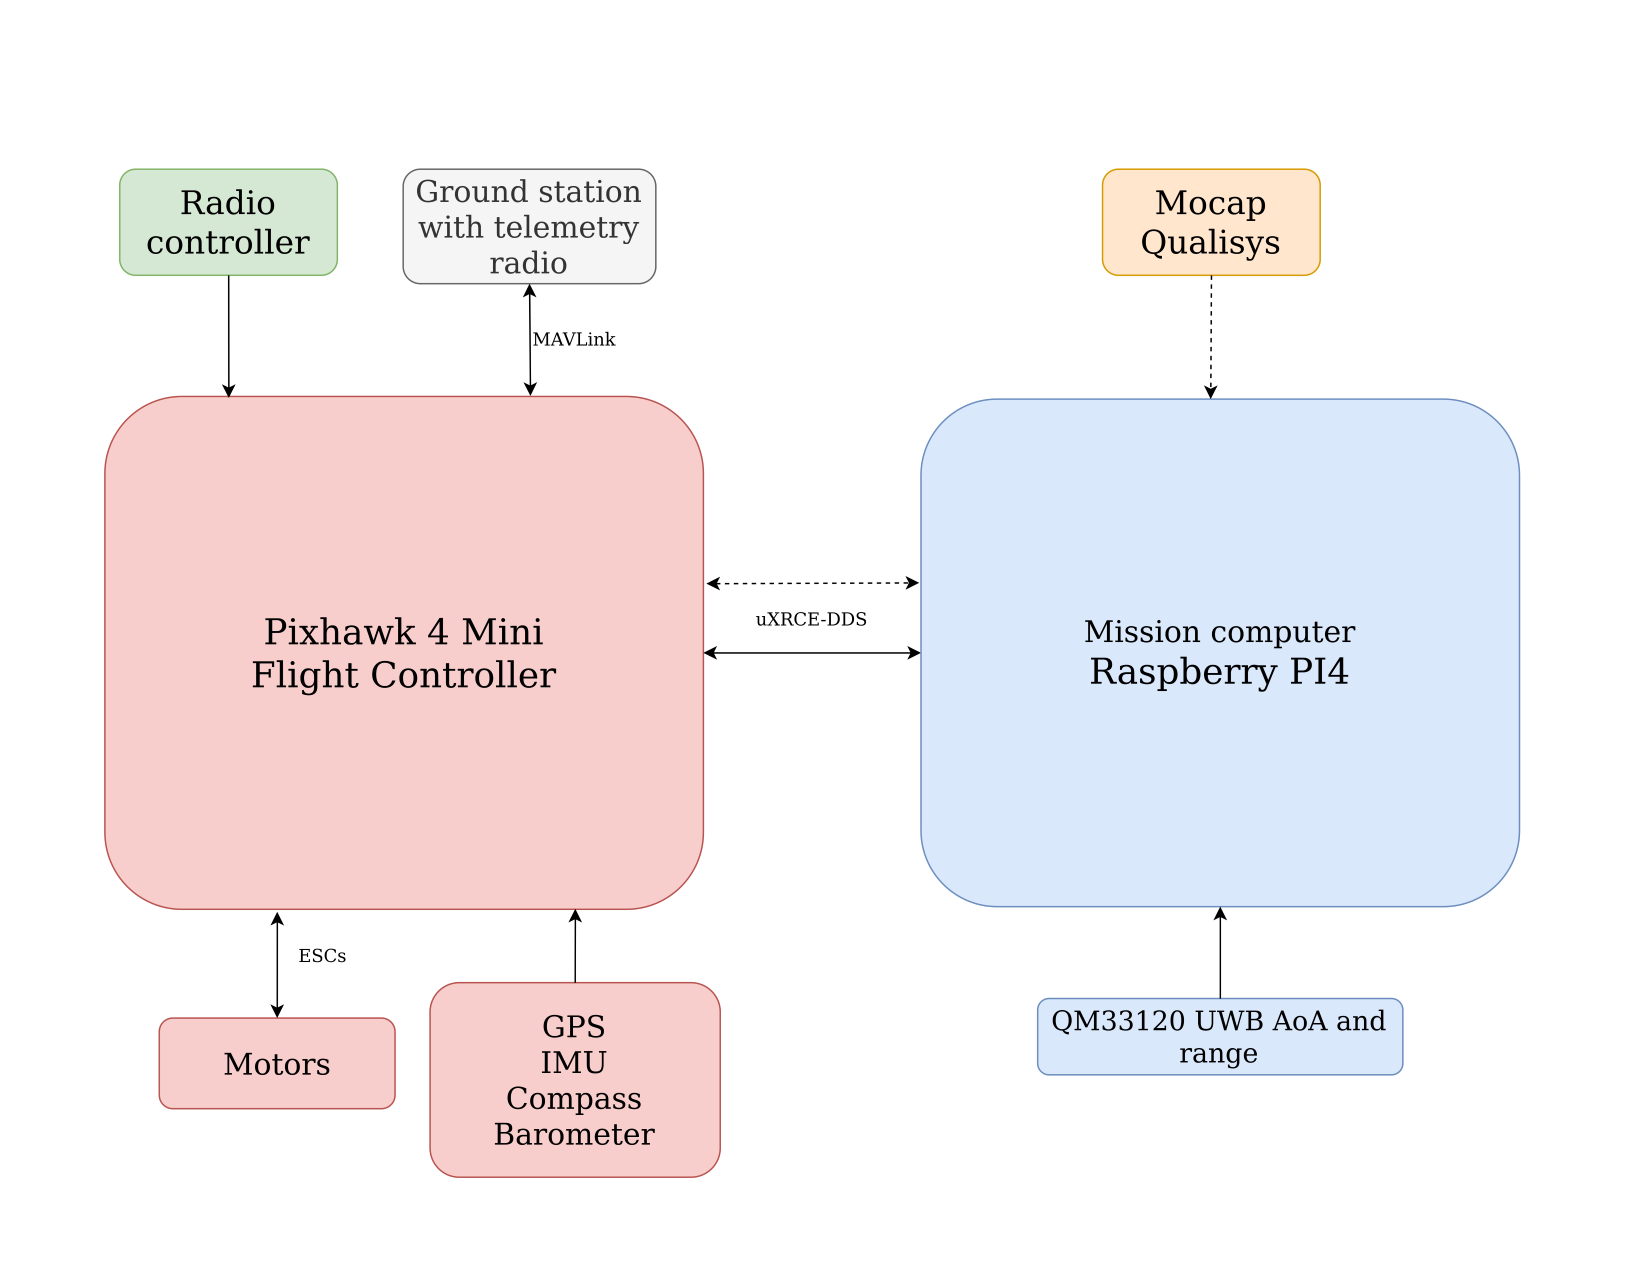
\includegraphics[width=0.45\textwidth]{images/FCA.png}
    \caption{Quadcopter architecture.}
    \label{ARC:fig_comp}
\end{figure}

\begin{figure}
    \centering
    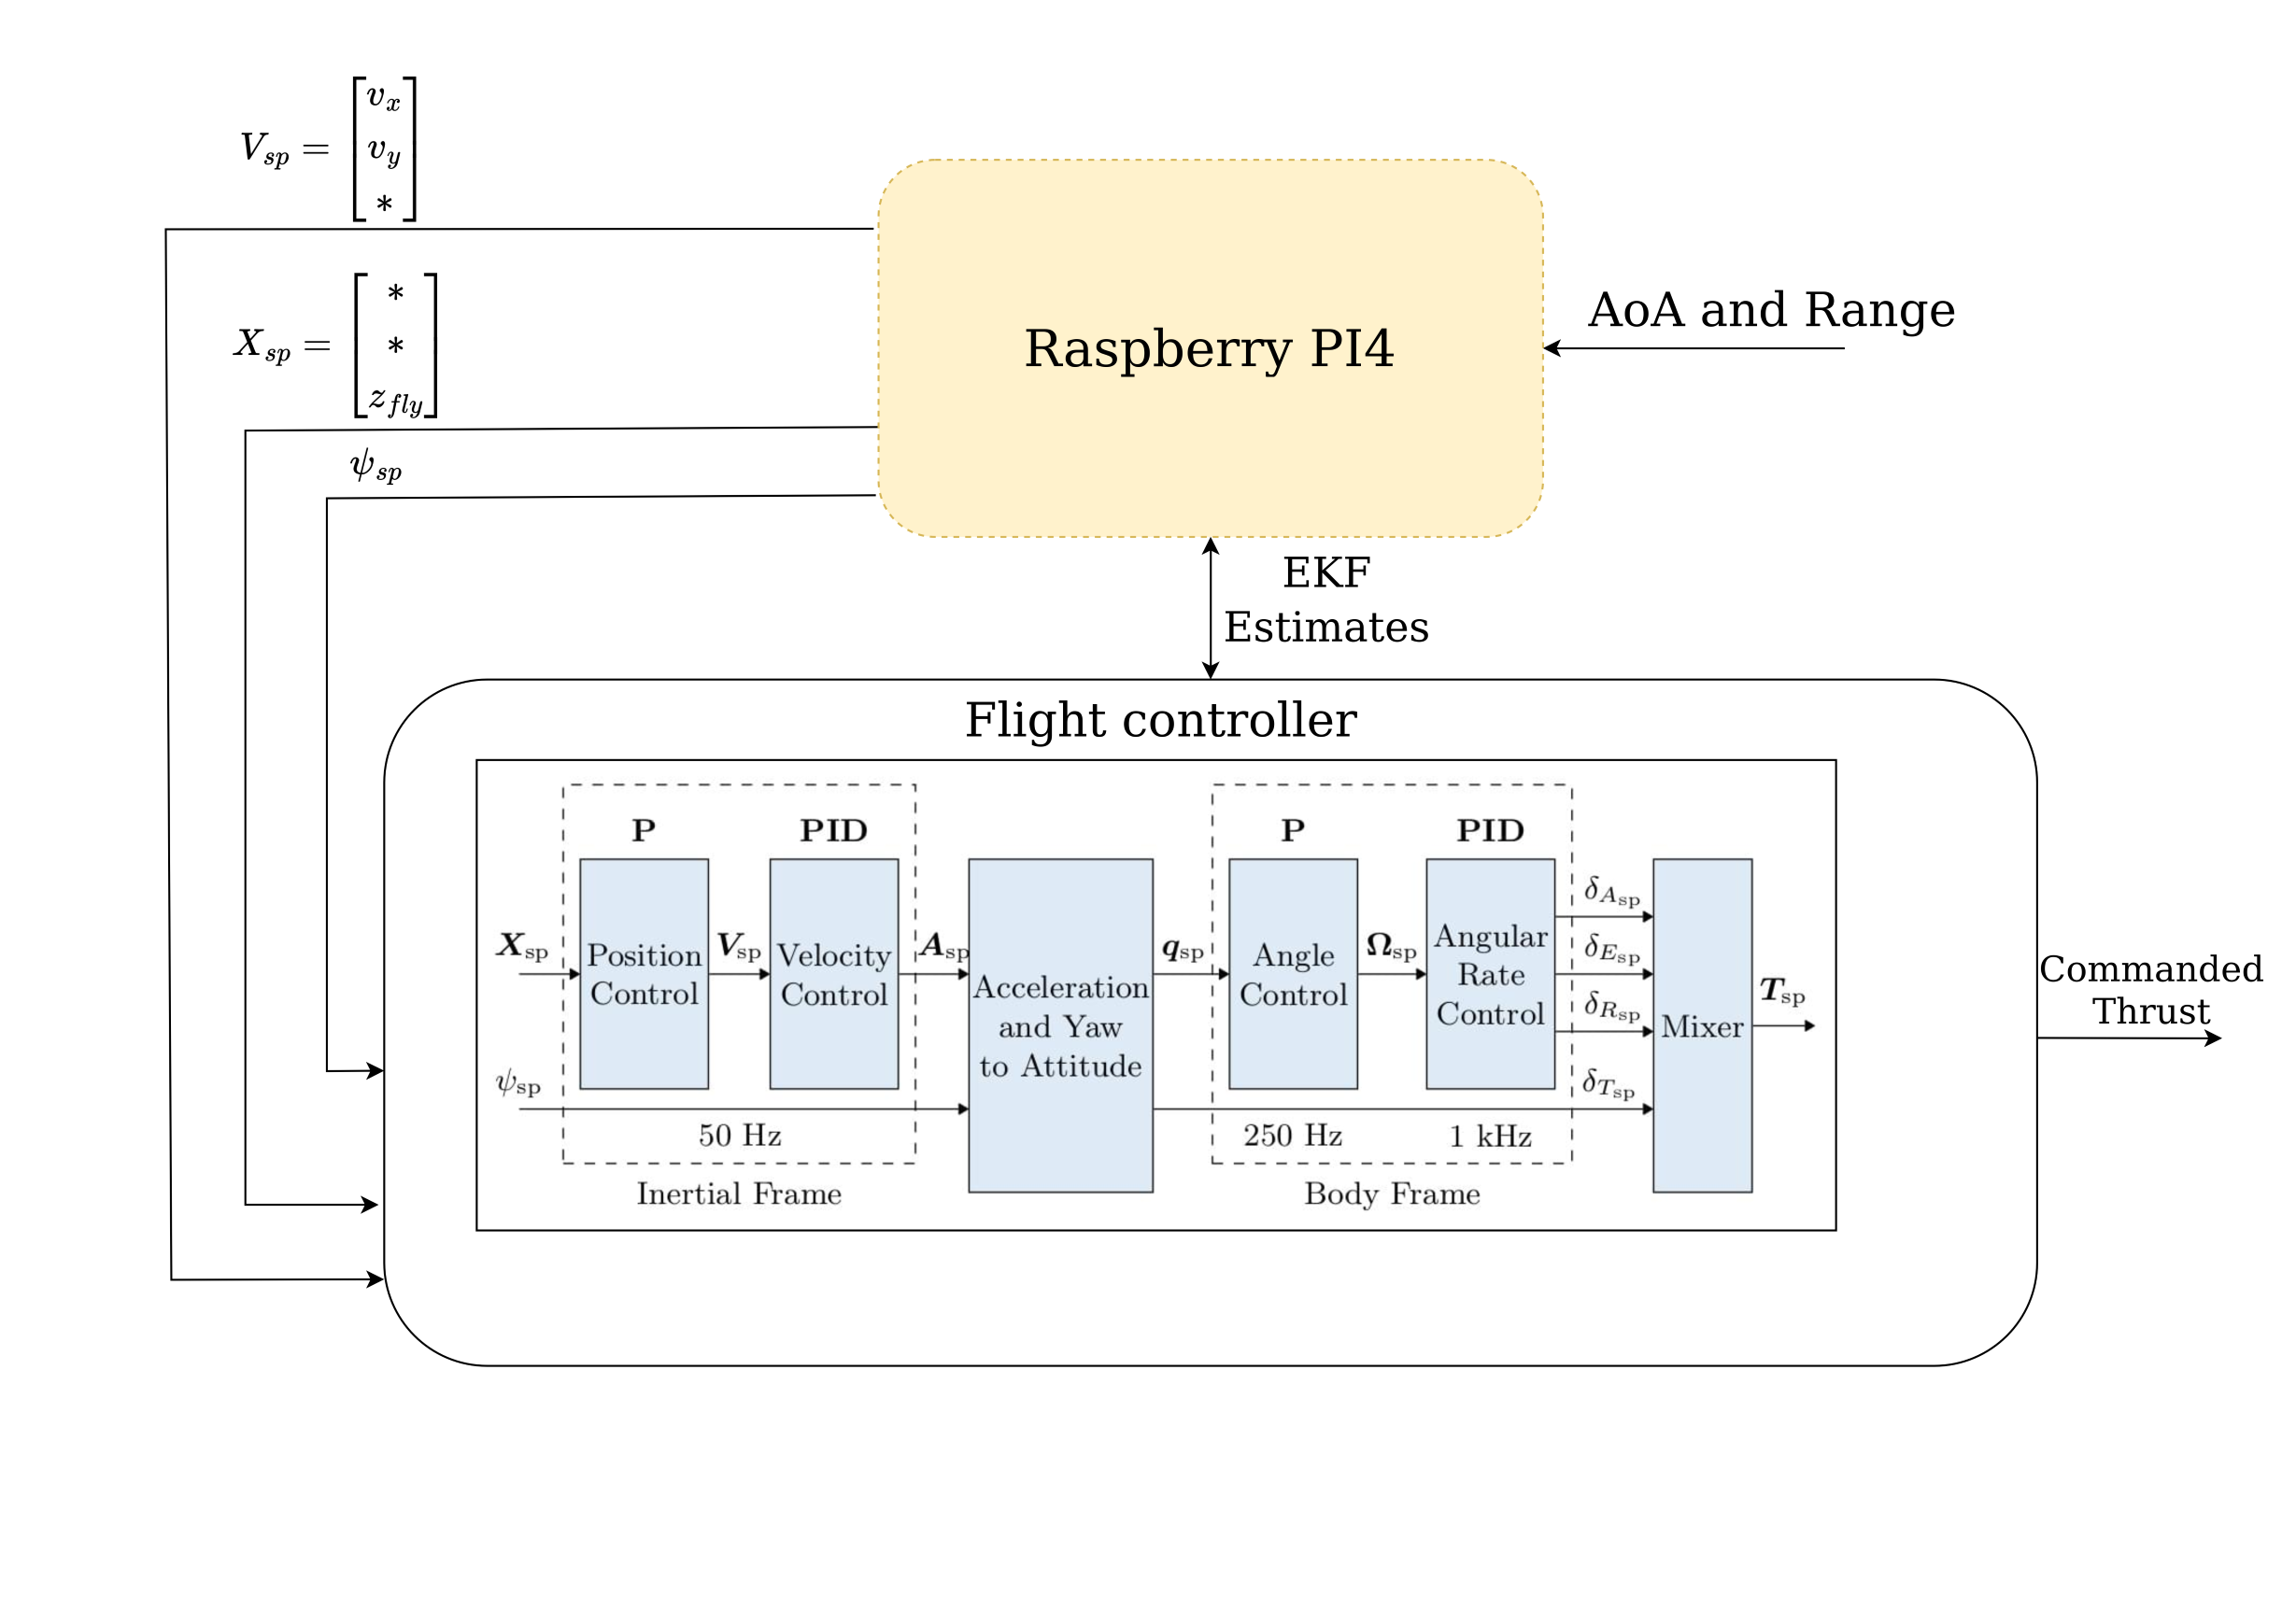
\includegraphics[width=0.45\textwidth]{images/Contr Diagram.png}
    \caption{Flight control loop: * stands for not controlled: if in \(X_{sp}\) it means that control computed starting from Velocity Control, if in \(V_{sp}\) computed by not empty Position Control input.}
    \label{ARC:fig_contr}
\end{figure}

In the proposed leader-follower application, the target carries a single antenna UWB transceiver while the chaser is a QAV250 quadcopter equipped with a Pixhawk4 Mini flight controller, a Raspberry Pi4 and a double antenna UWB transceiver that communicates through serial port to the mission computer, supplying to it range and angle of arrival of the target w.r.t. the drone.

\subsection{Quadcopter architecture}
The architecture and the interactions between the components of the vehicle are schematized in \autoref{ARC:fig_comp}.\\
The flight controller (FC) runs the PX4 Autopilot firmware, responsible for controlling propellers and for state estimates. The Raspberry using the received target location information and the drone state estimates, provides the control velocity setpoints, together with the yaw and the height setpoints (as explained in \autoref{control_law}), to the FC. The flight controller then, using a combination of nested P and PID controllers, converts the inputs in motor thrust commands (as depicted in figure \autoref{ARC:fig_contr}).\\

Since PX4 has the possibility of using a uXRCE-DDS middleware (a client running on the FC and an agent on the Raspberry) to allow uORB messages (that contains information such as command or veichle estimates and status) to be published and subscribed on a companion computer as they were ROS2 topics, the Raspberry can interact with the flight controller using these topics (better details about ROS2, topics and publishing/subscribing will be later exposed). The advantage of using the middleware ROS2 is a great flexibility, since all the devices connected to the same network can access to all the topics published, even those of the FC interfaced to the Raspberry. In our case this is particularly useful, in order to integrate Motion capture as the global reference for the UAV, as it will be explained later, and of course to send the FC control inputs.

\subsection{Target}
To ensure that the UWB tag keeps a constant height during the motion and to avoid possible dangerous situations that involves human beings during testing, as target we used a customized differential drive lawn-mower robot \autoref{ARC:fig:tag_photo}, with the UWB tag rigidly mounted on it. During our tests a person was in charge of driving this DDR with a radio controller.

\begin{figure}
    \centering
    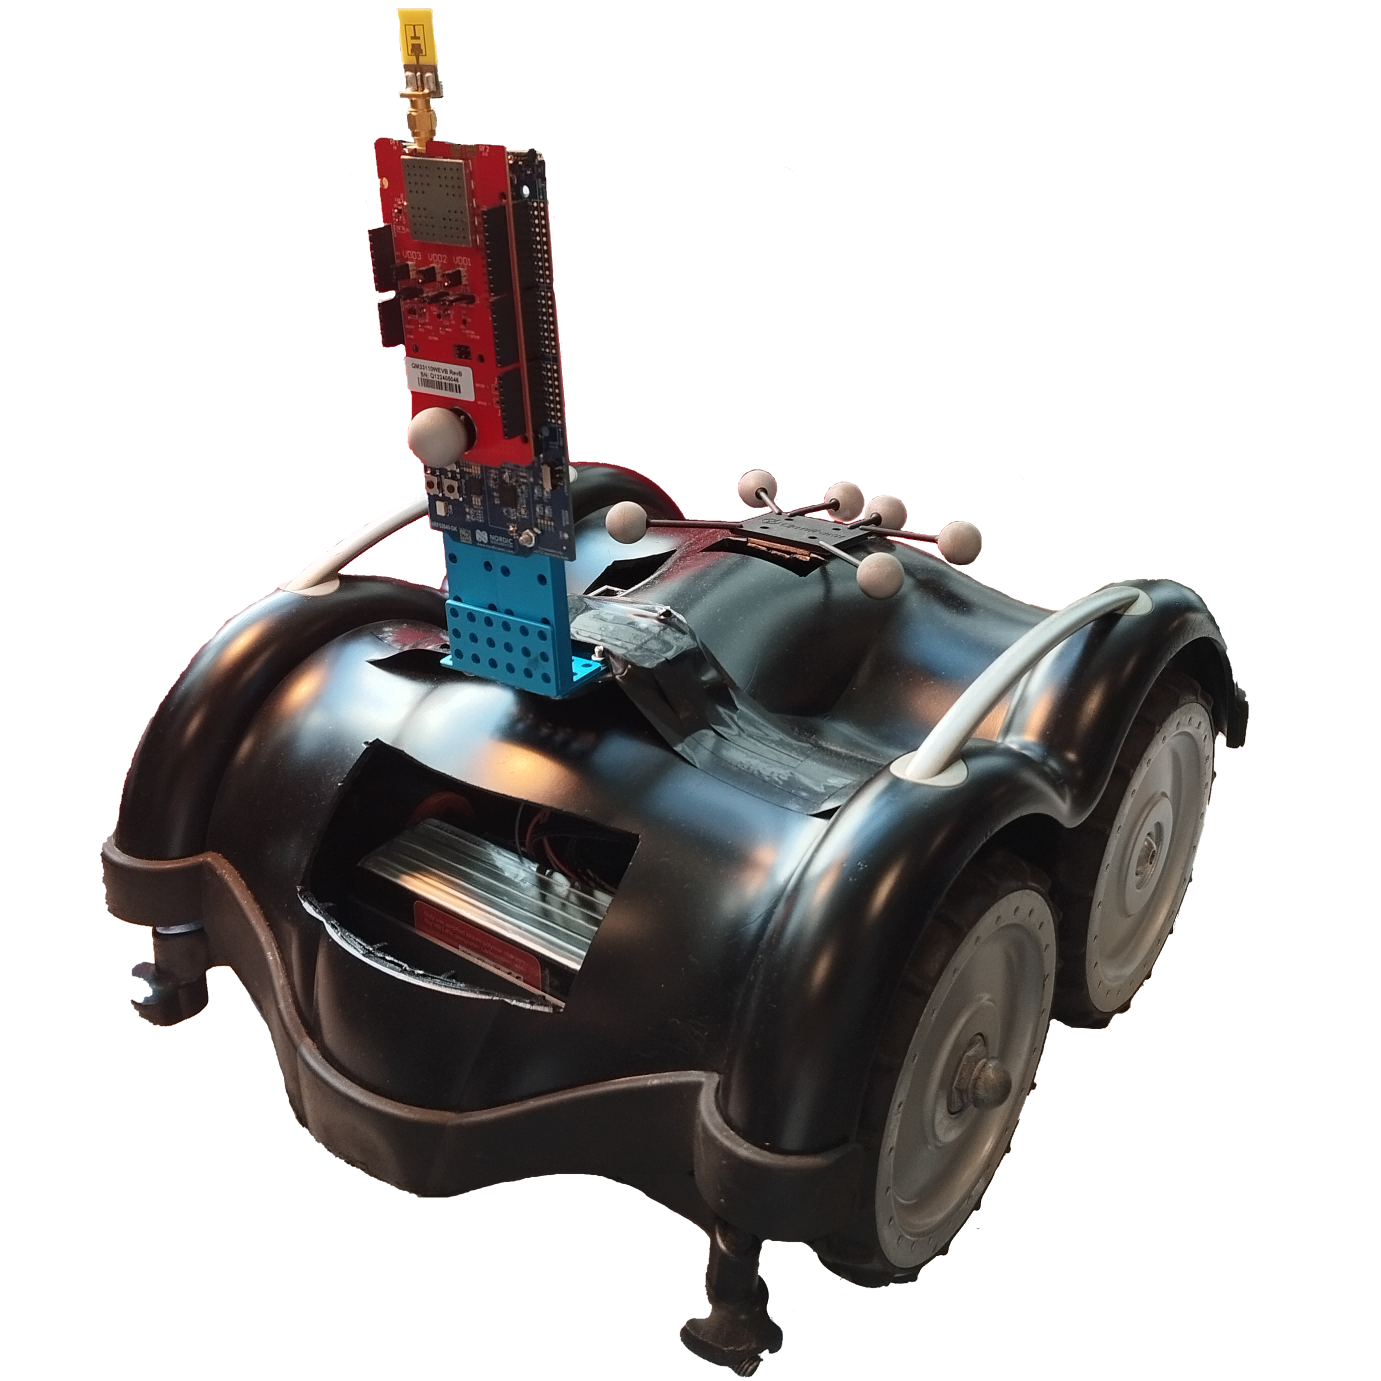
\includegraphics[width=0.4\textwidth]{images/target_reale_tagliato.png}
    \caption{DDR target. It is visible the mounted single antenna, as well as the presence of the Mocap markers, used to get its global position.}
    \label{ARC:fig:tag_photo}
\end{figure}

\subsection{Qualisys motion capture system}
In order to have a precise pose ground truth, we performed our tests indoor in a dedicated room with a system of seven Qualisys Arqus cameras installed. The system is able to precisely locate the reflective markers that can be mounted on the bodies to track, using the different views of the cameras. To track a body, a fixed configuration of at least 3 markers has to be mounted on it. However, to avoid possible troubles with marker occlusions, is suggested to place more markers. In our case, we tracked the target and the quadcopter to evaluate their motion. \\
Since in indoor GPS is not available, the quadcopter pose estimate, done by the MoCap, is used also as global pose, both in position and orientation. The way in which it is done will be explained in \autoref{Mocap details}. In addition we have disabled the compass and the barometer contribution to the vehicle's EKF, deactivating the related parameters in the flight controller firmware, since Mocap provides alone, a millimeter-level positioning precision. Beyond the uselessness, the reason of this deactivation lies in the indoor unreliability of these type measurements, due to environmental interference or misleading information (i.e. altitude and magnetic orientation have no meaning in the global reference frame of the Mocap lab).